\chapter{Architecture : base de données}

La base de donnée nous sert à sauvegarder les universités, les élèves et leurs affectations durant leurs études en cycle ingénieur. Elle nous permet aussi d'enregistrer des informations complémentaires, comme les commentaires sur les destinations, ou les documents administratifs des élèves par exemple.
\bigbreak
Notre base de donnée a reçu quelques changements mineurs depuis la remise du dernier rapport afin qu'elle soit sous forme 3NF. Ces problèmes ont pu êtres détectés grâce à la séance d'affectation effectuée sur l'application courant Janvier. Ceci n'a heureusement pas causé de problèmes pour les élèves du département INFO.

La base de donnée nous permet de respecter les spécifications suivantes :
\bigbreak
\begin{itemize}
	\item les identifiants et informations liées à un étudiant doivent être uniques;
	\item un étudiant peut faire autant de vœux qu'il le souhaite.
	\item l'affectation de l'élève est unique, et est donnée après l'acceptation du responsable RI (suite à la commission RI);
	\item les universités disposent d'un nombre de jetons variables, qui est ensuite réparti parmi les différents départements;
	\item lors de l'affectation, les jetons sont dépensés en fonction du département de l'élève;
	\item certaines informations devront être accessibles sur le site, vis à vis des destinations, vœux, classements ...
\end{itemize}
\bigbreak
Nous nous sommes particulièrement intéressés aux problématiques suivantes, afin d'assurer le bon fonctionnement de l'application :
\bigbreak
\begin{itemize}
	\item les étudiants sont rechargés depuis le CAS chaque année. L'application doit pouvoir déterminer quels étudiants ont redoublés ou reviennent d'une année de césure par exemple;
	\item l'algorithme d'affectation doit conserver le classement imbriqué (4A,3A), même quand certaines affectations sont faites manuellement au préalable.
\end{itemize}
\bigbreak
L'application est aujourd'hui fonctionnelle, mais nous restons à l'affût de bugs qui pourraient survenir. Un diagramme de la base de donnée est présent à la page suivante.

\newpage
\begin{figure}
	\centering
	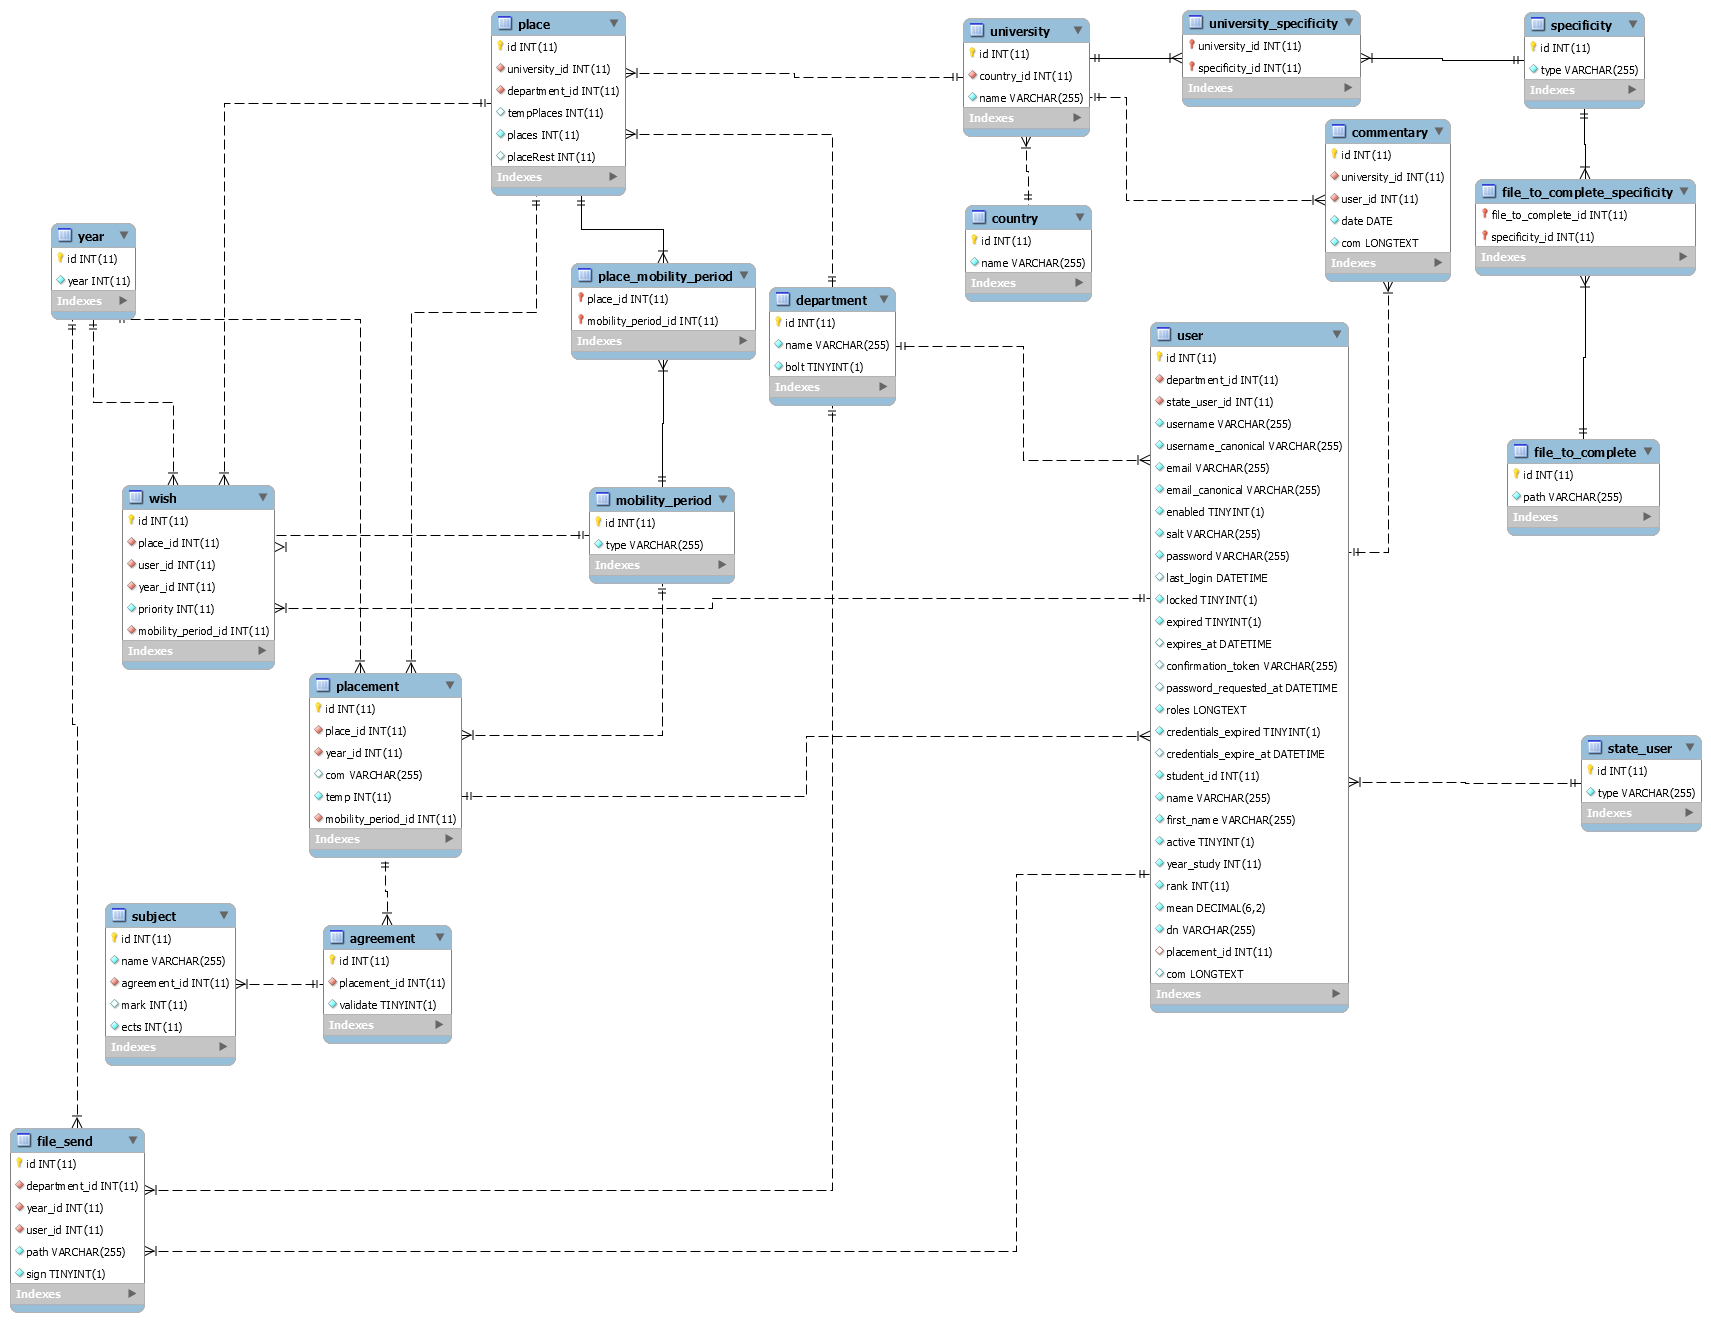
\includegraphics[scale=0.35,angle=90]{images/graph.png}
	\caption{Diagramme de l'architecture de la base de données}
\end{figure}
